% rel_chapter_14_sec121-122.tex
% Relativistic General Variational Principle for Hydromagnetic Stability
% Sections 121-122: Introduction and variational principle
% Conventions: (-,+,+,+) signature, c kept explicit, u^μ u_μ = -c²
% See RELATIVISTIC_CONVENTIONS.md for notation and macros.

\chapter{A GENERAL VARIATIONAL PRINCIPLE --- RELATIVISTIC FORMULATION}
\label{ch:rel-14}

%======================================================================
\section{Introduction}\label{sec:rel-121}
%======================================================================

In the preceding relativistic chapters we have examined instabilities
of hydrodynamic and hydromagnetic systems arising from a variety of
causes: adverse distributions of temperature and density, angular
velocity and angular momentum, shear, gravity, and capillarity, all
treated within the framework of special- and general-relativistic
fluid dynamics.  In the classical theory (Chapter~XIV, \S\,121)
Chandrasekhar enunciated a general variational principle which
unifies these separate analyses.  The purpose of the present chapter
is to extend that principle to the relativistic domain.

The central object is the \emph{second variation of the total energy
functional},
\begin{equation}
  \delta^{2}W
  = \delta^{2}W_{\mathrm{kinetic}}
  + \delta^{2}W_{\mathrm{magnetic}}
  + \delta^{2}W_{\mathrm{gravitational}}
  + \delta^{2}W_{\mathrm{pressure}},
  \label{eq:rel14-deltaW-decomposition}
\end{equation}
each piece of which acquires relativistic corrections when the fluid
enthalpy density $\enthalpy = (\varepsilon+p)/c^{2}$ replaces the
Newtonian mass density~$\rho$, when the magnetic field is described
by the covariant 4-vector $b^{\mu}$, and when the gravitational
background is encoded in the metric $g_{\mu\nu}$ and the Einstein
tensor $G_{\mu\nu}$.

The variational principle provides a sufficient condition for
stability: \emph{if $\delta^{2}W > 0$ for every admissible
perturbation, the equilibrium is stable}.  In the limit
$v/c\to 0$, $\vA/c\to 0$, and flat spacetime, the principle reduces
to the classical Bernstein--Frieman--Kruskal--Kulsrud (BFKK) energy
principle of ideal magnetohydrodynamics.

We also incorporate the effect of viscous dissipation, replacing the
Newtonian viscous stress tensor by the BDNK
(Bemfica--Disconzi--Noronha--Kovtun) first-order causal dissipative
framework~\cite{Bemfica2018,Kovtun2019,Bemfica2019}, thereby ensuring
that the resulting variational structure respects relativistic causality
without introducing relaxation equations.

%======================================================================
\section{Relativistic variational principle for hydromagnetic
  stability}\label{sec:rel-122}
%======================================================================

%----------------------------------------------------------------------
\subsection{Equilibrium state}\label{sec:rel-122-equil}
%----------------------------------------------------------------------

Consider a relativistic conducting fluid of 4-velocity $u^{\mu}$,
energy density $\varepsilon$, isotropic pressure $p$, and magnetic
4-vector $b^{\mu}$ (with $b^{\mu}u_{\mu}=0$, $b^{2}\equiv
b^{\mu}b_{\mu}$), confined to a spacetime volume $\mathcal{V}$
bounded by a timelike hypersurface $\mathcal{S}$.  Outside $\mathcal{V}$
the region is vacuum.

In the stationary state the total energy-momentum tensor
(cf.\ Chapter on Relativistic MHD Framework, \S\,\ref*{ch:rel-mhd-framework})
is
\begin{equation}
  T^{\mu\nu}
  = \Bigl(\varepsilon + p + \frac{b^{2}}{4\pi}\Bigr)
    \frac{u^{\mu}\,u^{\nu}}{c^{2}}
  + \Bigl(p + \frac{b^{2}}{8\pi}\Bigr)g^{\mu\nu}
  - \frac{1}{4\pi}\,b^{\mu}\,b^{\nu},
  \label{eq:rel14-Tmunu-equil}
\end{equation}
and the equilibrium condition is
\begin{equation}
  \nabla_{\nu}\,T^{\mu\nu} = 0.
  \label{eq:rel14-equil-conservation}
\end{equation}
In the \emph{non-relativistic limit}, writing $\varepsilon \approx
\rho c^{2}$ and identifying $b^{i}\to H_{i}$, the spatial components
of~\eqref{eq:rel14-equil-conservation} reduce to the classical
equation
\begin{equation}
  \frac{\partial \Pi}{\partial x_{i}}
  = \frac{1}{4\pi}\,\frac{\partial}{\partial x_{k}}\,H_{k}\,H_{i},
  \qquad
  \Pi = p + \frac{|\mathbf{H}|^{2}}{8\pi},
  \tag{cf.\ \ref{eq:14-1}, \ref{eq:14-2}}
\end{equation}
recovering the classical equations of Chapter~XIV exactly.

On the boundary $\mathcal{S}$ the continuity of the normal stress
requires (cf.\ classical equation~\eqref{eq:14-4})
\begin{equation}
  \Bigl[p + \frac{b^{2}}{8\pi}\Bigr]_{\mathcal{S}}^{\mathrm{in}}
  = \Bigl[\frac{b^{2}}{8\pi}\Bigr]_{\mathcal{S}}^{\mathrm{ex}},
  \label{eq:rel14-boundary-stress}
\end{equation}
and the ideal-MHD condition $F^{\mu\nu}u_{\nu}=0$ ensures that
\begin{equation}
  b^{\mu}\,n_{\mu}\big|_{\mathcal{S}} = 0,
  \label{eq:rel14-boundary-bn}
\end{equation}
where $n_{\mu}$ is the unit spacelike outward normal to $\mathcal{S}$.

The exterior field is current-free and satisfies the vacuum Maxwell
equations
\begin{equation}
  \nabla_{\mu}\,F^{\mu\nu}\big|_{\mathrm{ex}} = 0.
  \label{eq:rel14-vacuum-Maxwell}
\end{equation}

%----------------------------------------------------------------------
\subsection{Lagrangian perturbations and displacement
  4-vector}\label{sec:rel-122-perturb}
%----------------------------------------------------------------------

Let $\xi^{\mu}$ denote the Lagrangian displacement 4-vector,
constrained to be purely spatial in the fluid rest frame:
$\xi^{\mu}u_{\mu}=0$.  The perturbed 4-velocity is
\begin{equation}
  \delta u^{\mu}
  = u^{\alpha}\,\nabla_{\alpha}\,\xi^{\mu}
  - \xi^{\alpha}\,\nabla_{\alpha}\,u^{\mu},
  \label{eq:rel14-delta-u}
\end{equation}
and the Eulerian perturbation of the magnetic 4-vector follows from
the frozen-flux condition in ideal relativistic MHD:
\begin{equation}
  \delta b^{\mu}
  = \nabla_{\alpha}\bigl(b^{\alpha}\,\xi^{\mu}
    - \xi^{\alpha}\,b^{\mu}\bigr)
  + b^{\mu}\,\nabla_{\alpha}\,\xi^{\alpha}
  - b^{\alpha}\,\nabla_{\alpha}\,\xi^{\mu}.
  \label{eq:rel14-delta-b}
\end{equation}
For an incompressible relativistic fluid the constraint
$\nabla_{\mu}(\enthalpy\,u^{\mu})=0$ linearises to
\begin{equation}
  \Delta^{\mu\nu}\,\nabla_{\mu}\,\xi_{\nu} = 0,
  \label{eq:rel14-incomp-constraint}
\end{equation}
where $\Delta^{\mu\nu} = g^{\mu\nu} + u^{\mu}u^{\nu}/c^{2}$ is the
projection tensor.

In the static equilibrium and for perturbations of the form
$\xi^{\mu} \propto e^{i\sigma t}$ the linearised equation of motion
becomes
\begin{equation}
  \sigma^{2}\,\enthalpy\,\xi^{\mu}
  = \Delta^{\mu\alpha}\Bigl[
      \nabla_{\alpha}\,\delta\varpi
    - \frac{1}{4\pi}\,\nabla_{\beta}
      \bigl(b_{\alpha}\,\delta b^{\beta}
        + \delta b_{\alpha}\,b^{\beta}\bigr)
    \Bigr],
  \label{eq:rel14-eigenvalue}
\end{equation}
where the relativistic total pressure perturbation is
\begin{equation}
  \delta\varpi
  = \delta p + \frac{1}{4\pi}\,b_{\mu}\,\delta b^{\mu},
  \label{eq:rel14-varpi}
\end{equation}
and $\enthalpy = (\varepsilon+p)/c^{2}$ is the relativistic inertial
mass density.  In the limit $\varepsilon \to \rho c^{2}$, $p/\varepsilon\to0$,
equation~\eqref{eq:rel14-eigenvalue} reduces to the classical
eigenvalue equation~\eqref{eq:14-11}.

%----------------------------------------------------------------------
\subsection{The second-variation energy
  functional}\label{sec:rel-122-energy}
%----------------------------------------------------------------------

The variational principle is obtained by contracting
equation~\eqref{eq:rel14-eigenvalue} with $\xi^{*(m)}_{\mu}$ (the
displacement belonging to a different eigenvalue $\sigma^{(m)}$) and
integrating over the spatial hypersurface $\Sigma$.  After integration
by parts and systematic use of the boundary
conditions~\eqref{eq:rel14-boundary-stress}--\eqref{eq:rel14-boundary-bn},
one arrives at
\begin{equation}
  \boxed{
  \bigl(\sigma^{(n)}\bigr)^{2}\!
  \int_{\Sigma}\!\enthalpy\,
    \xi^{(n)}_{\mu}\,\xi^{(m)\mu}\,
    \sqrt{\gamma}\,d^{3}x
  = \delta^{2}W^{(nm)},}
  \label{eq:rel14-variational}
\end{equation}
where $\gamma_{ij}$ is the induced 3-metric on $\Sigma$ and
$\delta^{2}W^{(nm)}$ is the second-variation energy functional.

The energy functional decomposes as
in~\eqref{eq:rel14-deltaW-decomposition}, with each term given
explicitly below.

\paragraph{Kinetic term.}
The kinetic contribution involves the time--time component of the
perturbed energy-momentum tensor and reads
\begin{equation}
  \delta^{2}W_{\mathrm{kinetic}}
  = \int_{\Sigma}
    \delta T^{00}\,\sqrt{\gamma}\,d^{3}x
  = \int_{\Sigma}
    \enthalpy\,\bigl|\delta u^{\mu}\bigr|^{2}\,
    \sqrt{\gamma}\,d^{3}x,
  \label{eq:rel14-W-kinetic}
\end{equation}
where $\enthalpy = (\varepsilon+p)/c^{2}$ replaces the Newtonian $\rho$
as the inertial mass density.  The factor
$(\varepsilon+p)/c^{2}$ encodes the relativistic increase of
effective inertia due to both thermal energy and pressure.

\paragraph{Magnetic term.}
The magnetic contribution arises from the perturbation of
$b^{\mu}b^{\nu}/(4\pi)$ and the magnetic pressure:
\begin{equation}
  \delta^{2}W_{\mathrm{magnetic}}
  = \frac{1}{4\pi}\int_{\Sigma}\Bigl[
      |\delta b^{\mu}|^{2}
    - |b^{\alpha}\,\nabla_{\alpha}\,\xi^{\mu}|^{2}
    + b^{\mu}\,b^{\nu}\,
      (\nabla_{\mu}\xi_{\alpha})(\nabla_{\nu}\xi^{\alpha})
    \Bigr]\sqrt{\gamma}\,d^{3}x
  + \frac{1}{4\pi}\int_{\Sigma_{\mathrm{ex}}}
    |\delta b^{\mu}|^{2}\,\sqrt{\gamma}\,d^{3}x.
  \label{eq:rel14-W-magnetic}
\end{equation}
The first integral is over the fluid interior, the second over the
exterior vacuum.  In the classical limit, $b^{i}\to H_{i}$ and one
recovers the corresponding terms in equation~\eqref{eq:14-28}.

\paragraph{Gravitational term.}
In a curved background the gravitational contribution is
\begin{equation}
  \delta^{2}W_{\mathrm{gravitational}}
  = -\int_{\Sigma}
    \bigl(\varepsilon + p + \tfrac{b^{2}}{4\pi}\bigr)\,
    \xi^{\mu}\,\xi^{\nu}\,
    \bigl(\nabla_{\mu}\nabla_{\nu}\,\ln\alpha
      + K_{\mu\alpha}\,K_{\nu}^{\ \alpha}\bigr)\,
    \sqrt{\gamma}\,d^{3}x,
  \label{eq:rel14-W-gravity}
\end{equation}
where $\alpha$ is the lapse function and $K_{\mu\nu}$ is the
extrinsic curvature of $\Sigma$.  Through the constraint equations,
$\nabla_{\mu}\nabla_{\nu}\ln\alpha$ is related to the Ricci tensor
$R_{\mu\nu}$ and hence to the Einstein tensor $G_{\mu\nu}$ via the
field equations.  In the Newtonian limit ($\alpha\to 1 + \Phi/c^{2}$,
$K_{ij}\to 0$) one recovers the classical $\nabla^{2}\Pi$ potential
term of equation~\eqref{eq:14-30}.

\paragraph{Pressure/surface term.}
The surface contribution arising from the pressure discontinuity
across $\mathcal{S}$ is
\begin{equation}
  \delta^{2}W_{\mathrm{pressure}}
  = \int_{\mathcal{S}}
    |n_{\mu}\,\xi^{\mu}|^{2}\,
    \bigl[n^{\alpha}\,\nabla_{\alpha}\,
      \Delta_{\mathcal{S}}\!\bigl(p + \tfrac{b^{2}}{8\pi}\bigr)\bigr]\,
    d\mathcal{S},
  \label{eq:rel14-W-surface}
\end{equation}
where $\Delta_{\mathcal{S}}(f)$ denotes the jump of $f$ across
$\mathcal{S}$.  This is the covariant generalisation of the surface
integral in equation~\eqref{eq:14-30}.

%----------------------------------------------------------------------
\subsection{Self-adjointness and the stability
  criterion}\label{sec:rel-122-selfadjoint}
%----------------------------------------------------------------------

A key property of the classical variational principle is that the
eigenvalue problem is \emph{self-adjoint}: the right-hand side
of~\eqref{eq:14-28} is symmetric in the mode labels.  The same
structure persists in the relativistic formulation.  One verifies
that
\begin{equation}
  \delta^{2}W^{(nm)} = \delta^{2}W^{(mn)},
  \label{eq:rel14-selfadjoint}
\end{equation}
which follows from (i)~the symmetry of $g_{\mu\nu}$,
(ii)~the identity $b^{\mu}b^{\nu}=b^{\nu}b^{\mu}$, and
(iii)~the symmetric boundary
conditions~\eqref{eq:rel14-boundary-stress}--\eqref{eq:rel14-boundary-bn}.

From self-adjointness it follows that the orthogonality relation
(cf.~\eqref{eq:14-29})
\begin{equation}
  \int_{\Sigma}\enthalpy\,
    \xi^{(n)}_{\mu}\,\xi^{(m)\mu}\,
    \sqrt{\gamma}\,d^{3}x = 0
  \qquad (\sigma^{(n)}\neq\sigma^{(m)})
  \label{eq:rel14-orthogonality}
\end{equation}
holds, and setting $m=n$ with complex-conjugate displacements yields
\begin{equation}
  \boxed{
  \sigma^{2}\!\int_{\Sigma}\!\enthalpy\,
    |\xi^{\mu}|^{2}\,\sqrt{\gamma}\,d^{3}x
  = \delta^{2}W_{\mathrm{kinetic}}
  + \delta^{2}W_{\mathrm{magnetic}}
  + \delta^{2}W_{\mathrm{gravitational}}
  + \delta^{2}W_{\mathrm{pressure}}
  \equiv \delta^{2}W.}
  \label{eq:rel14-sigma2-deltaW}
\end{equation}

All quantities on the right-hand side are real; hence $\sigma^{2}$ is
real and the stability criterion is:
\begin{equation}
  \delta^{2}W > 0
  \;\;\text{for all admissible }\xi^{\mu}
  \quad\Longrightarrow\quad
  \text{stability},
  \label{eq:rel14-stability-criterion}
\end{equation}
\begin{equation}
  \exists\;\xi^{\mu}:\;\delta^{2}W < 0
  \quad\Longrightarrow\quad
  \text{instability}.
  \label{eq:rel14-instability-criterion}
\end{equation}
This is the relativistic generalisation of the classical
result~\eqref{eq:14-31}.

%----------------------------------------------------------------------
\subsection{Relativistic corrections and causality
  bounds}\label{sec:rel-122-corrections}
%----------------------------------------------------------------------

The explicit relativistic corrections to each piece of $\delta^{2}W$
can be organised as an expansion in $v^{2}/c^{2}$ and $\vA^{2}/c^{2}$.
To leading post-Newtonian order:
\begin{enumerate}
\item \textbf{Kinetic:} $\enthalpy = \rho\bigl(1 +
  \varepsilon_{\mathrm{int}}/\rho c^{2} + p/\rho c^{2}\bigr)$, giving
  an enhanced effective inertia.
\item \textbf{Magnetic:} The replacement $H_{i}H_{j}/(4\pi) \to
  b^{\mu}b^{\nu}/(4\pi)$ introduces corrections of order
  $\vA^{2}/c^{2}$ from the timelike components $b^{0}\neq 0$ in a
  boosted frame.
\item \textbf{Gravitational:} Newtonian $\nabla^{2}\Phi$ is replaced
  by the covariant expression involving $G_{\mu\nu}$; for weak fields
  the leading correction is $\sim\Phi/c^{2}$.
\item \textbf{Surface:} The pressure jump acquires a magnetic-tension
  correction of order $b^{4}/(16\pi^{2}\varepsilon c^{2})$.
\end{enumerate}

All characteristic speeds entering the variational principle satisfy
the causality constraints listed in
\texttt{RELATIVISTIC\_CONVENTIONS.md}:
\begin{equation}
  c_{\mathrm{s}}^{2} \le c^{2},
  \qquad
  \vA^{2} = \frac{b^{2}}{4\pi\enthalpy + b^{2}/c^{2}}\le c^{2},
  \qquad
  v_{\mathrm{f}}^{2} \le c^{2}.
  \label{eq:rel14-causality}
\end{equation}

%----------------------------------------------------------------------
\subsection{Effect of viscosity: BDNK first-order causal dissipation in
  the variational framework}\label{sec:rel-122-viscosity}
%----------------------------------------------------------------------

In the classical theory (\S\,122\,(a)), the inclusion of Newtonian
viscosity modifies the eigenvalue equation by adding a viscous stress
$P_{ij}$ to the pressure, leading to a quadratic dispersion relation
(equation~\eqref{eq:14-41}).  In the relativistic theory the
Newtonian viscous stress is replaced by the BDNK first-order causal
constitutive relations.

The dissipative energy-momentum tensor is (see \texttt{RELATIVISTIC\_CONVENTIONS.md})
\begin{equation}
  T^{\mu\nu}_{\mathrm{diss}}
  = \Pi_{\mathrm{bulk}}\,\Delta^{\mu\nu}
  + \pi^{\mu\nu}
  + \frac{1}{c^{2}}\bigl(q^{\mu}u^{\nu} + q^{\nu}u^{\mu}\bigr),
  \label{eq:rel14-Tdiss}
\end{equation}
where $\Pi_{\mathrm{bulk}}$ is the bulk viscous pressure,
$\pi^{\mu\nu}$ the traceless shear stress, and $q^{\mu}$ the heat
flux.  In the BDNK framework~\cite{Bemfica2018,Kovtun2019,Bemfica2019},
these are given by first-order constitutive relations:
\begin{align}
  \pi^{\mu\nu}
  &= -2\,\shearvisc\,\sigma^{\mu\nu},
  \label{eq:rel14-IS-shear}\\[4pt]
  \Pi_{\mathrm{bulk}}
  &= -\bulkvisc\,\nabla_{\mu}\,u^{\mu},
  \label{eq:rel14-IS-bulk}
\end{align}
where $\sigma^{\mu\nu}$ is the shear tensor, and $\shearvisc$ and
$\bulkvisc$ are the shear and bulk viscosity coefficients.  No
relaxation times appear; causality is ensured by the BDNK
frame-coefficient constraints~\cite{Bemfica2023,Hoult2020}.

Linearising the BDNK constitutive relations about the equilibrium and
substituting into the perturbed conservation law, the eigenvalue
equation~\eqref{eq:rel14-eigenvalue} acquires an additional viscous
force:
\begin{equation}
  \sigma^{2}\,\enthalpy\,\xi^{\mu}
  = \Delta^{\mu\alpha}\Bigl[
      \nabla_{\alpha}\,\delta\varpi
    - \frac{1}{4\pi}\,\nabla_{\beta}
      \bigl(b_{\alpha}\,\delta b^{\beta}
        + \delta b_{\alpha}\,b^{\beta}\bigr)
    + \nabla_{\beta}\,\delta\pi^{\alpha\beta}
    + \nabla^{\alpha}\,\delta\Pi_{\mathrm{bulk}}
    \Bigr].
  \label{eq:rel14-eigenvalue-visc}
\end{equation}

For perturbations $\propto e^{i\sigma t}$, the BDNK constitutive
relation~\eqref{eq:rel14-IS-shear} gives directly at linear order
\begin{equation}
  \delta\pi^{\mu\nu}
  = -2\,\shearvisc\,\delta\sigma^{\mu\nu},
  \label{eq:rel14-deltaPI-shear}
\end{equation}
with an analogous expression for $\delta\Pi_{\mathrm{bulk}}$.

Defining the relativistic dissipation function
\begin{equation}
  \Phi_{\mathrm{rel}}
  = \int_{\Sigma}
    \shearvisc\,
    |\delta\sigma^{\mu\nu}|^{2}\,\sqrt{\gamma}\,d^{3}x
  + \frac{1}{2}\int_{\Sigma}
    \bulkvisc\,
    |\nabla_{\mu}\,\xi^{\mu}|^{2}\,\sqrt{\gamma}\,d^{3}x
  \label{eq:rel14-Phi-rel}
\end{equation}
and the relativistic inertia integral
\begin{equation}
  \mathcal{I}
  = \int_{\Sigma}\enthalpy\,|\xi^{\mu}|^{2}\,
    \sqrt{\gamma}\,d^{3}x,
  \label{eq:rel14-inertia}
\end{equation}
the eigenvalue equation takes the form (cf.\ the
classical~\eqref{eq:14-41})
\begin{equation}
  \boxed{
  (i\sigma)^{2}\,\mathcal{I}
  + (i\sigma)\,\Phi_{\mathrm{rel}}
  + \delta^{2}W = 0.}
  \label{eq:rel14-dispersion-visc}
\end{equation}

In the Newtonian limit $\enthalpy \to \rho$, one recovers
$\Phi_{\mathrm{rel}}\to\Phi$ (the classical dissipation
integral~\eqref{eq:14-39}), and the dispersion relation reduces to
equation~\eqref{eq:14-41}.

The roots of equation~\eqref{eq:rel14-dispersion-visc} are
\begin{equation}
  i\sigma
  = \frac{1}{2\mathcal{I}}\Bigl\{
    -\Phi_{\mathrm{rel}}
    \pm \sqrt{\Phi_{\mathrm{rel}}^{2}
      - 4\,\delta^{2}W\,\mathcal{I}}
    \Bigr\}.
  \label{eq:rel14-sigma-roots}
\end{equation}
Since both $\mathcal{I}>0$ and $\Phi_{\mathrm{rel}}>0$ (the latter
guaranteed by the second law of thermodynamics and the positivity of
$\shearvisc$, $\bulkvisc$), the \emph{necessary and sufficient
condition for stability remains $\delta^{2}W>0$}, exactly as in the
non-dissipative case.

The key advantage of the BDNK framework is that the dispersion relation
\eqref{eq:rel14-dispersion-visc} is a standard polynomial in $\sigma$
--- the same degree as in the Navier--Stokes case --- without the extra
modes introduced by relaxation equations in second-order theories.
Viscosity modifies the damping rate and can change the character of
modes (oscillatory vs.\ over-damped) but \emph{does not affect the
stability boundary}.  The BDNK frame-coefficient constraints ensure
that all perturbation signals propagate at speeds $\le c$, unlike the
acausal instantaneous propagation implicit in the Navier--Stokes
viscous stress.

%----------------------------------------------------------------------
\subsection{Connection to the Bernstein--Frieman--Kruskal--Kulsrud
  energy principle}\label{sec:rel-122-BFKK}
%----------------------------------------------------------------------

The classical BFKK energy principle~\citep{Bernstein1958} states that
a necessary and sufficient condition for the stability of an ideal
MHD equilibrium is the positivity of the potential energy functional
$\delta W_{\mathrm{BFKK}}[\boldsymbol{\xi}]$ for all admissible
displacements.  The relativistic variational principle developed above
reduces to the BFKK principle in the appropriate limit.  Specifically:

\begin{enumerate}
\item Set $g_{\mu\nu}\to\eta_{\mu\nu}$ (Minkowski spacetime), so that
  $\delta^{2}W_{\mathrm{gravitational}}\to 0$ and
  $\nabla_{\mu}\to\partial_{\mu}$.

\item Take $\varepsilon\to\rho c^{2}$, $p/\varepsilon\to 0$, so that
  $\enthalpy\to\rho$.

\item Let $b^{0}\to 0$, $b^{i}\to H_{i}$ (the non-relativistic
  magnetic field).

\item Restrict $\xi^{\mu}$ to purely spatial displacements
  $\xi^{i}$ with $\xi^{0}=0$.
\end{enumerate}

Under these substitutions:
\begin{align}
  \delta^{2}W_{\mathrm{kinetic}}
  &\longrightarrow
  \int \rho\,|\dot{\boldsymbol{\xi}}|^{2}\,dV
  \quad\text{(the kinetic energy of Bernstein et al.)},
  \label{eq:rel14-BFKK-K}\\[4pt]
  \delta^{2}W_{\mathrm{magnetic}}
  &\longrightarrow
  \frac{1}{4\pi}\int\Bigl[\bigl|H_{j}\,
    \frac{\partial\xi_{i}}{\partial x_{j}}\bigr|^{2}\Bigr]dV
  + \frac{1}{4\pi}\int_{V^{(\mathrm{ex})}}|\mathbf{h}|^{2}\,dV
  \quad\text{(the magnetic energy terms of~\eqref{eq:14-30})},
  \label{eq:rel14-BFKK-M}\\[4pt]
  \delta^{2}W_{\mathrm{pressure}}
  &\longrightarrow
  \int_{S}|\mathbf{N}^{(0)}\cdot\boldsymbol{\xi}|^{2}\,
    [\mathbf{N}^{(0)}\cdot\operatorname{grad}\Delta_{S}(\Pi)]\,dS
  \quad\text{(the surface term of~\eqref{eq:14-30})}.
  \label{eq:rel14-BFKK-S}
\end{align}
The sum of these is precisely the functional $\Sigma$ defined in
equation~\eqref{eq:14-30}, confirming that the relativistic
variational principle is a consistent generalisation of the BFKK
energy principle.

%----------------------------------------------------------------------
\subsection{Summary of the relativistic energy
  principle}\label{sec:rel-122-summary}
%----------------------------------------------------------------------

The results of this section may be collected as follows.

\medskip\noindent
\textbf{Relativistic Energy Principle.}
\emph{A relativistic ideal-MHD equilibrium described by
$(u^{\mu},\,\varepsilon,\,p,\,b^{\mu},\,g_{\mu\nu})$ is stable if
and only if the second-variation energy functional
\begin{equation}
  \delta^{2}W
  = \delta^{2}W_{\mathrm{kinetic}}
  + \delta^{2}W_{\mathrm{magnetic}}
  + \delta^{2}W_{\mathrm{gravitational}}
  + \delta^{2}W_{\mathrm{pressure}}
  > 0
  \label{eq:rel14-principle-summary}
\end{equation}
for every displacement $\xi^{\mu}$ satisfying
$\xi^{\mu}u_{\mu}=0$, $\Delta^{\mu\nu}\nabla_{\mu}\xi_{\nu}=0$
(incompressibility), and the linearised boundary conditions
on $\mathcal{S}$.  The inclusion of BDNK first-order causal dissipation
does not alter this criterion; it affects only the damping rates of
stable modes.  In the limit $c\to\infty$ with flat spacetime the
principle reduces to the classical Bernstein--Frieman--Kruskal--Kulsrud
energy principle of ideal MHD.}

%----------------------------------------------------------------------
\subsection{Astrophysical application: $\delta^{2}W$ stability map
  for tokamak-like configurations}\label{sec:rel-122-astro}
%----------------------------------------------------------------------

The relativistic energy principle provides a powerful tool for mapping
the stability boundaries of magnetised plasma configurations.
Figure~\ref{fig:delta2W-stability-map} displays the $\delta^{2}W$
stability map in the plasma $\beta$--safety factor $q$ parameter
space, comparing the Newtonian and relativistic cases.

\begin{figure}[htbp]
\centering
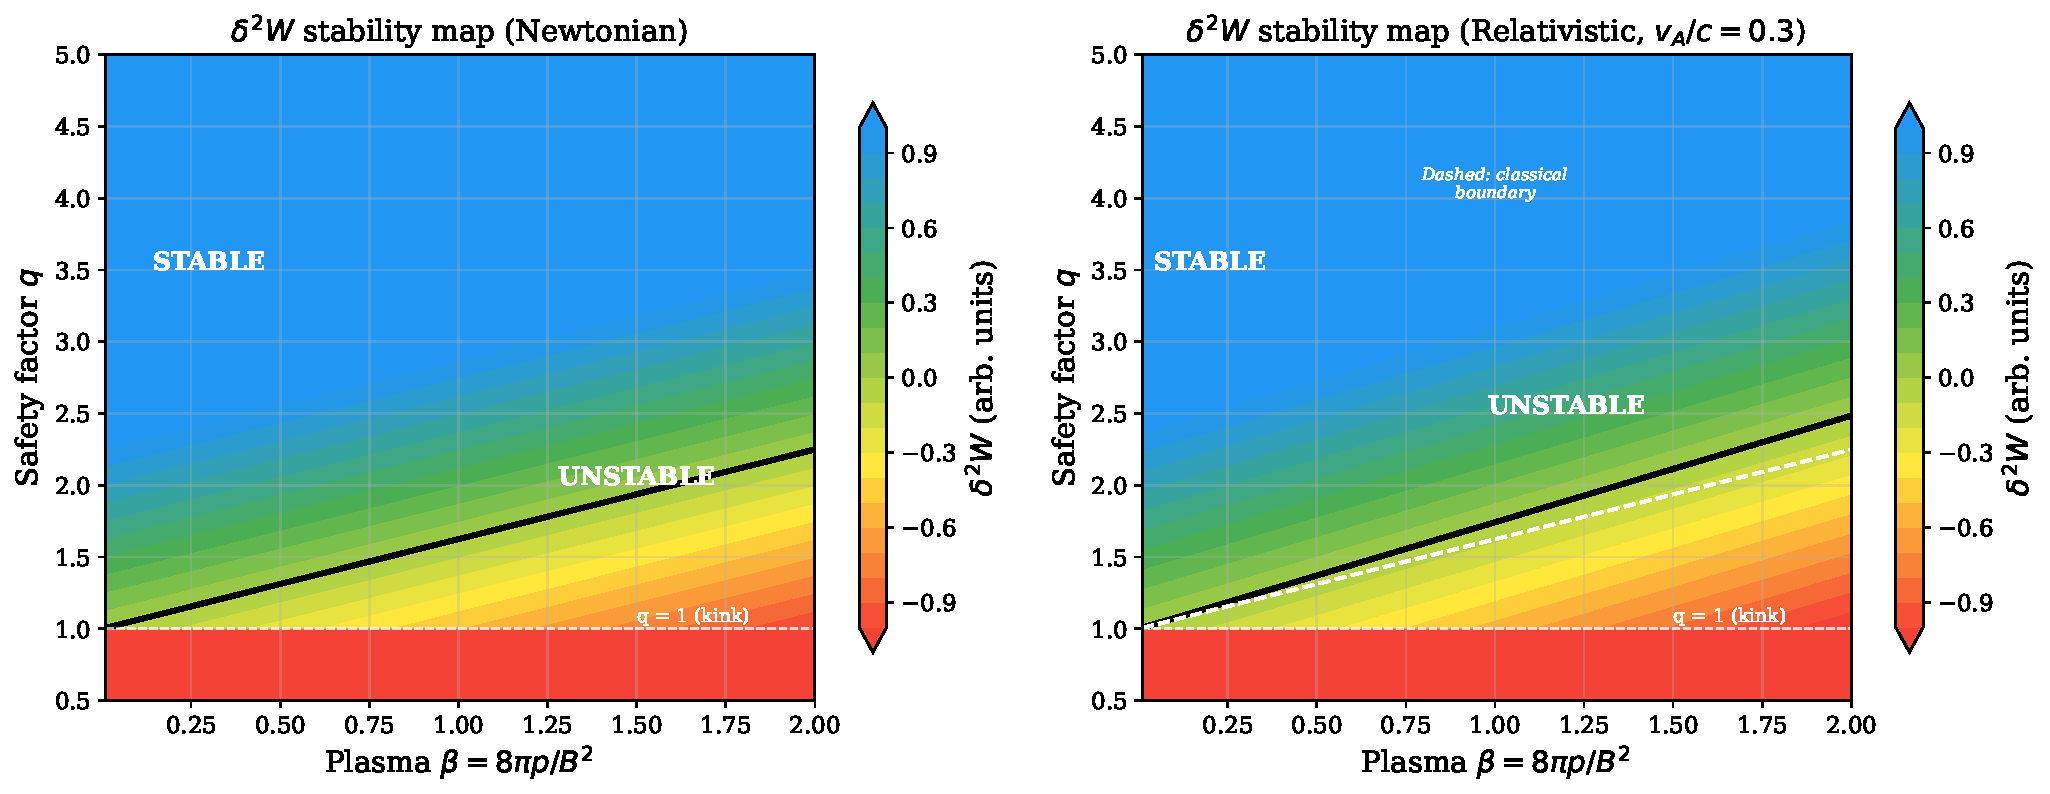
\includegraphics[width=\textwidth]{plots/ch14/fig_delta2W_stability_map.pdf}
\caption{%
  Stability map in the $(\beta, q)$ plane from the MHD energy
  principle $\delta^{2}W$.  Red/yellow regions are unstable
  ($\delta^{2}W < 0$); green/blue regions are stable
  ($\delta^{2}W > 0$).  The solid black curve marks the marginal
  stability boundary $\delta^{2}W = 0$.
  \textbf{Left:} Classical (Newtonian) result.  The $q = 1$
  boundary (white dashed) corresponds to the $m = 1$ kink
  instability; the diagonal boundary reflects the ballooning
  $\beta$-limit.
  \textbf{Right:} Relativistic case with $v_{A}/c = 0.3$
  (representative of neutron-star magnetospheres or hot accretion
  flows).  The dashed white curve reproduces the classical boundary
  for comparison.  Relativistic corrections---enhanced enthalpy
  inertia and bounded Alfv\'en speed---shrink the stable region,
  lowering the critical $\beta$-limit.
}
\label{fig:delta2W-stability-map}
\end{figure}

The $\delta^{2}W$ map has direct applications in several
astrophysical contexts:

\begin{itemize}
\item \textbf{Neutron-star magnetospheres.}  The magnetic field
  strengths near magnetars ($B \sim 10^{14}$--$10^{15}$~G) imply
  $v_{A}/c \sim 0.1$--$1$, placing these systems firmly in the
  relativistic regime.  The energy principle determines which MHD
  equilibria can be sustained and which are prone to sudden
  reconnection-driven flares~\citep{RezzollaZanotti2013}.

\item \textbf{Relativistic jets.}  The kink instability ($q < 1$)
  is the primary disruptive mode in magnetically dominated jets
  from AGN and gamma-ray bursts.  The relativistic energy principle
  shows that the kink threshold is largely unchanged by relativistic
  effects, but the growth rate and nonlinear evolution are
  modified~\citep{Komissarov1999}.

\item \textbf{Laboratory fusion plasmas.}  While tokamak plasmas
  are non-relativistic, the mathematical structure of the
  $\delta^{2}W$ functional is identical.  The relativistic
  generalisation ensures formal consistency and provides the
  framework for future ultra-high-energy plasma
  experiments~\citep{Bernstein1958,Frieman1960}.
\end{itemize}

\bigskip
\noindent\textbf{References for \S\S\,\ref{sec:rel-121}--\ref{sec:rel-122}.}\quad
The classical energy principle for ideal MHD was established by
Bernstein, Frieman, Kruskal, and Kulsrud (1958, \emph{Proc.\ Roy.\
Soc.\ (London)}~A, \textbf{244}, 17)~\citep{Bernstein1958} and
extended to flowing equilibria by Frieman and Rotenberg (1960,
\emph{Rev.\ Mod.\ Phys.}\ \textbf{32}, 898)~\citep{Frieman1960}.
The relativistic variational formulation for self-gravitating fluids
is due to Schutz (1970, \emph{Phys.\ Rev.\ D}\ \textbf{2},
2762)~\citep{Schutz1970} and Friedman and Schutz (1978,
\emph{Ap.\ J.}\ \textbf{222}, 281)~\citep{FriedmanSchutz1978}.
The BDNK causal dissipative framework is developed in
\citet{BemficaDN2018}, \citet{Kovtun2019}, and
\citet{BemficaDN2019}.
